\chapter{Observace, měření a reprezentace}
K pozorování meteorů a jejich záznamu se v současnosti používají tři přístupy: fotografické snímky, videozáznamy a radarová měření.

Ve všech třech přístupech je cílem sledovat a zaznamenávat celou oblohu nebo alespoň její velkou část. Například u fotografického přístupu se používá rybí oko \cite{ceplecha} -- čočka nebo objektiv, který je schopný zobrazit celou oblohu na jeden snímek. Cenou za takto širokoúhlý snímek je velké zkreslení obrazu, to lze ale pro účely měření matematicky odstranit \cite{ceplecha}.

\smallskip

Radarová měření využívají skutečnosti, že plyn ionizovaný průletem meteoroidu dobře odráží radiové vlny s frekvencí $24\:\text{MHz}$ \cite{radiosurvey}. Za použití radiového vysílače a několika přijímaču ve známých vzájemných vzdálenostech lze z okamžiků zrcadlového odrazu na jednotlivých přijímačích (maxima přijímaného signálu) určit trajektorii meteoru \cite{radiosurvey}. Rychlost letu meteoru se pak určí z Dopplerova jevu, jelikož dochází k difrakci radiových vln na pohybující se hraně (čelní části meteoru), a tato difrakce je závislá na rychlosti této hrany \cite{radiosurvey}.

\smallskip

Fotografické snímky a videozáznamy jsou z hlediska měření velmi blízké: Videozáznam je v principu pouze série fotografií, v minulém století se ale využívalo spíše opačného přístupu, kdy se několik fotografických záběrů zaznamenalo na jeden snímek \cite{ceplecha}. Oba přístupy tedy dávají průběh polohy (a případně i luminosity) meteoru v čase. Konkrétně pro metody identifikace meteorických rojů potřebujeme právě dráhu (polohu) a rychlost meteoru \cite{ceplecha}, abychom zjistili orbitální dráhu meteoroidu. Důkladněji se procesu zpracování fotografických snímků budeme věnovat v sekci \ref{sec:photography}.

\section{Elementy dráhy}\label{sec:orbit}
Orbitální dráhy jsou v prvním přiblížení elipsy, které jsou nakloněné v prostoru. Jedním z ohniskových bodů je vždy těžiště (Sluneční) soustavy, pro určení dráhy tedy stačí 5 parametrů \cite{astro}.

\medskip

Dva z parametrů popisují tvar elispy; její velikost a excentricitu \cite{astro}. \textit{Excentricita} $e$ náleží do intervalu $\left[0,1\right)$,\footnote{Excentricita může být také $=1$ pro parabolické a $>1$ pro hyperbolické dráhy. \ask{Otevřené, předpokládám, ignorujeme, protože by patřily do sporadického pozadí automaticky (nemají mateřský objekt ve Sluneční soustavě).}} a udává, jak blízká kružnici tato dráha je (viz obrázek \ref{img:orbit:ellipse}).

\begin{figure}[ht]
    \centering
    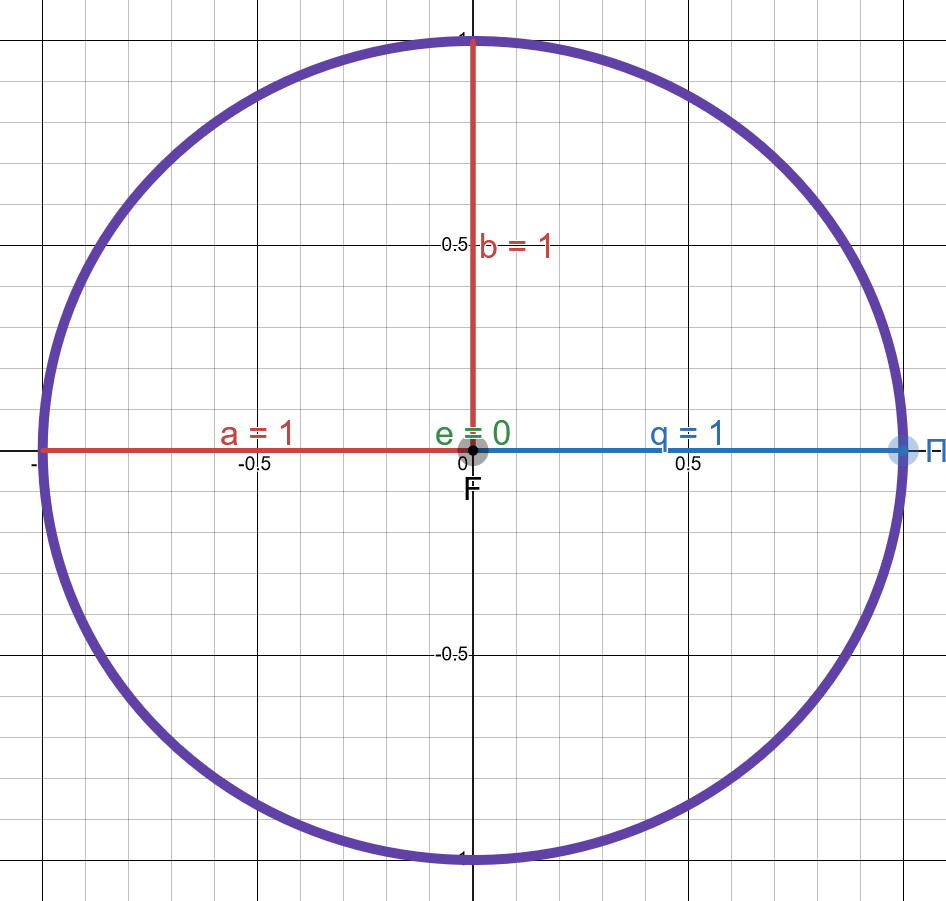
\includegraphics[width=0.5\linewidth]{img/ellipse-e00.png}\hfill
    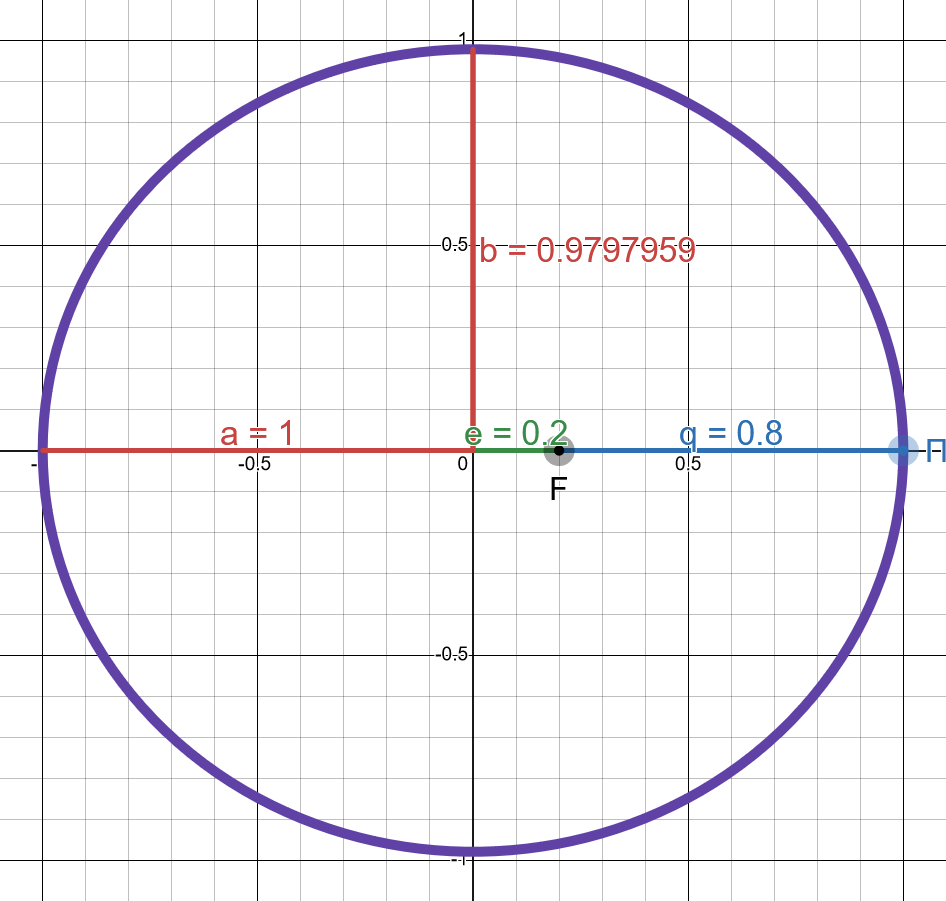
\includegraphics[width=0.5\linewidth]{img/ellipse-e02.png}\vfill
    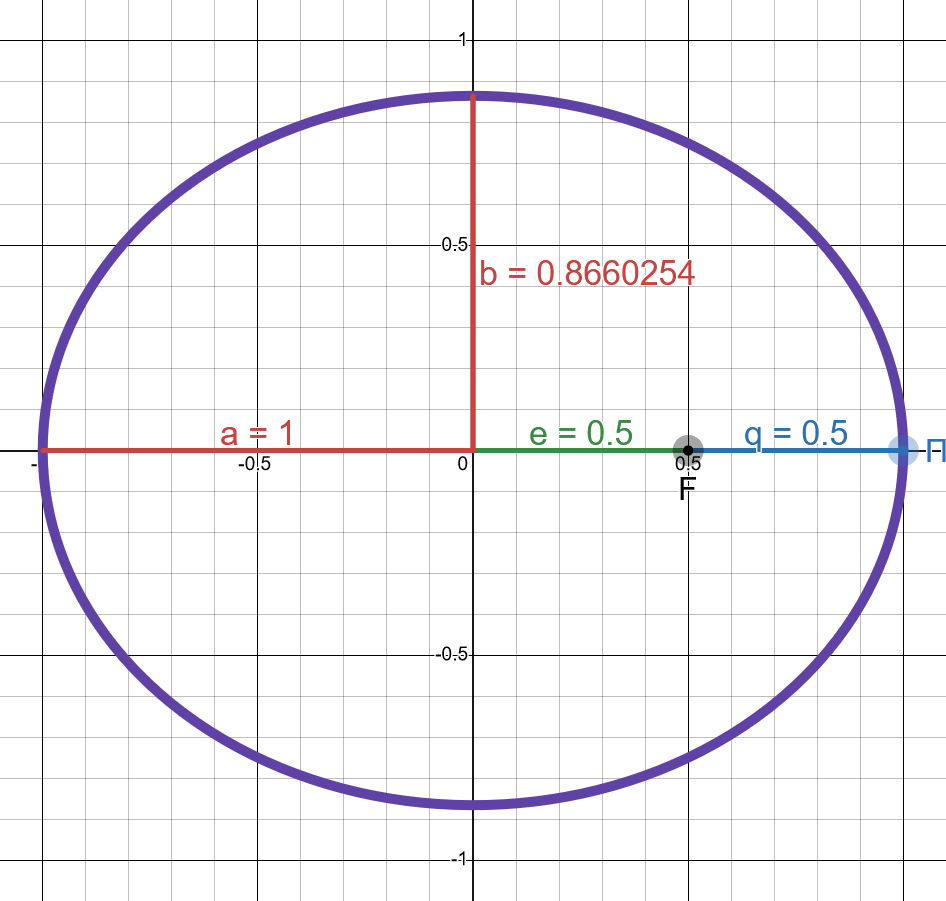
\includegraphics[width=0.5\linewidth]{img/ellipse-e05.png}\hfill
    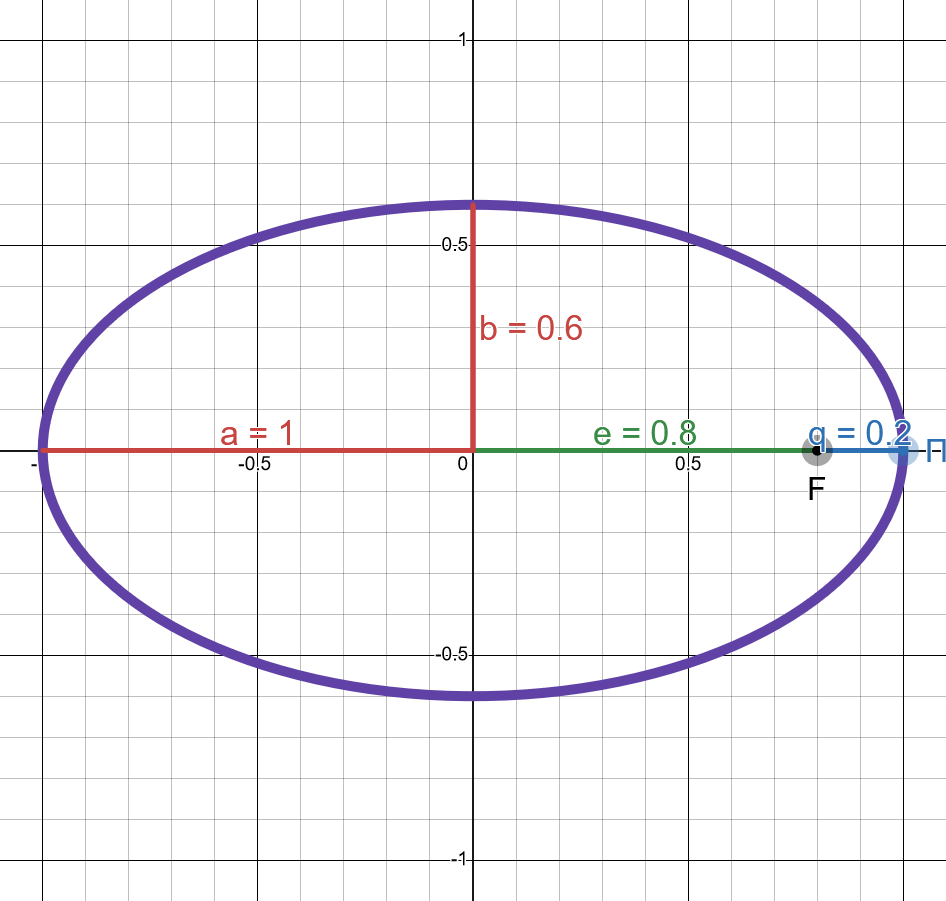
\includegraphics[width=0.5\linewidth]{img/ellipse-e08.png}
    \caption[Vliv lineární excentricity $e$ na tvar elipsy]{Vliv lineární excentricity $e$ na tvar elipsy\\{\small (zdroj: vlastní zpracování)}}
    \label{img:orbit:ellipse}
\end{figure}

Pro určení velikosti používáme buďto \textit{délku hlavní poloosy} $a$ nebo \textit{vzdálenost perihelia} $q$ (efektivně vzdálenost okraje elipsy od ohniska). Jejich vztah ilustruje obrázek \ref{img:orbit:ellipse} a mezi oběma lze převádět pomocí rovnice \cite{ceplecha}
$$
    q=a(1-e)\text{.}
$$

\smallskip

Zbylé tři parametry určují natočení elipsy v prostoru. Jedná se o obdobu Eulerových úhlů, jsou ovšem definované vůči Slunci a ekliptice. Tyto úhly jsou znázorněny v obrázku \ref{img:orbit:elements} a slovně se jedná o
\begin{itemize}
    \item \textit{inklinaci} $i$, která udává úhel mezi rovinou ekliptiky a rovinou elipsy \cite{astro},
    \item \textit{délku vzestupného uzlu} $\Omega$, která udává heliocentrickou ekliptikální délku bodu, ve kterém dráha protíná rovinu ekliptiky při průletu z jihu (tzv. \textit{vzestupný uzel}, \NorthNode) \cite{astro}, a
    \item \textit{argument perihelia} $\omega$, úhel, ve kterém se nachází perihelium, měřený od úsečky spojující Slunce a vzestupný uzel \cite{astro}.
\end{itemize}
Tyto úhly se aplikují jako rotace na rovinu ekliptiky s počátkem ve středu Slunce.

\begin{figure}[ht]
    \centering
    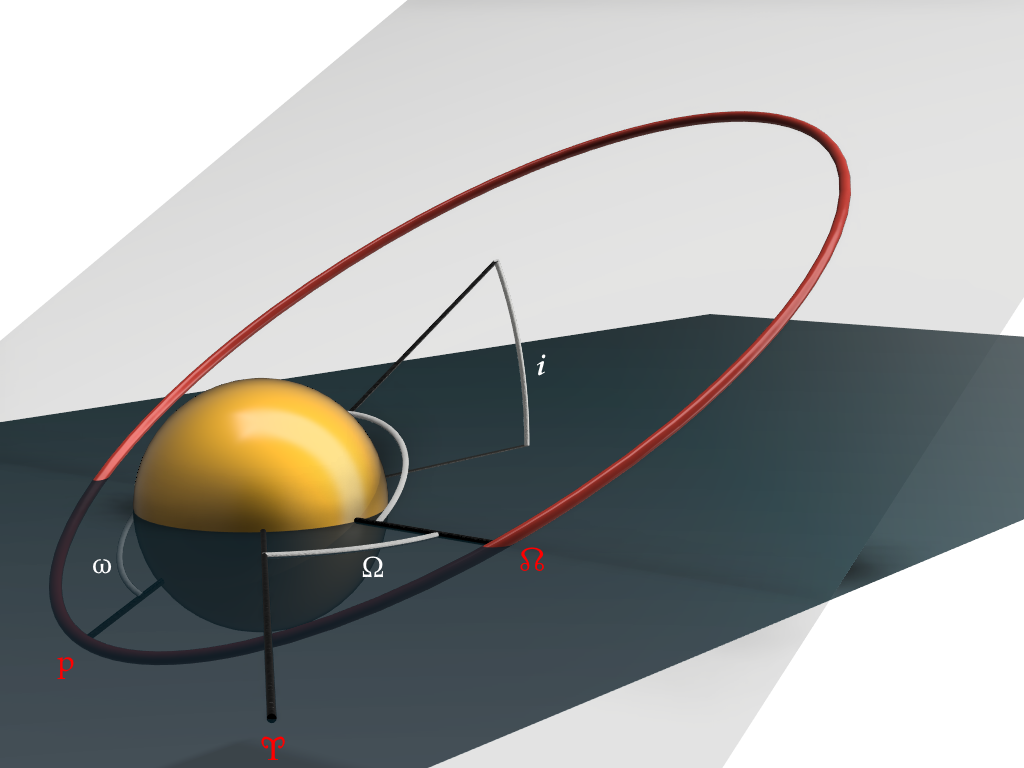
\includegraphics[width=0.8\linewidth]{img/orbit-elements-marked.png}
    \caption[Ilustrace významu elementů dráhy $i$, $\Omega$ a $\omega$]{
    Ilustrace významu elementů dráhy $i$, $\Omega$ a $\omega$\\
    {\small (zdroj: vlastní zpracování, \cite{astro})}
    }
    \label{img:orbit:elements}
\end{figure}

\medskip

Na takto definované dráze se ještě můžeme setkat se souřadnicí zvanou \textit{pravá anomálie} $\nu$. Ta již nespecifikuje dráhu, nýbrž polohu objektu na své dráze, a v meteodách identifikace meteorických rojů se vyskytuje jen zřídka. Udává se jako úhel měřený od spojnice Slunce a perihelia ke spojnici Slunce a objektu \cite{astro}.

\section{Fotografická měření}\label{sec:photography}
Úkolem astrometrických měření meteorů je zjistit elementy dráhy meteoroidu před tím, než se setkal s atmosférou Země. Vše ale začíná na fotografii nebo videozáznamu průletu meteoru atmosférou.

Budeme popisovat techniku měření používanou pro fotografická měření, kde máme fotoaparát s rybím okem pro zachycení celé oblohy a clonou, která s pevnou periodou (několikrát za vteřinu) zakrývá detektor nebo fotografický film, čímž zachytí časovou závislost pohybu meteoru. \todo{Bude-li obrázek, přidat a popsat.} Pro video je postup prakticky identický, hůře se ale ilustruje.

\medskip

Mějme stanice \textbf{A} a \textbf{B} ležící na zeměpisné šířce $\varphi_\mathbf{A}$ resp. $\varphi_\mathbf{B}$ a zeměpisné délce $\lambda_\mathbf{A}$ resp. $\lambda_\mathbf{B}$, kde je umístěn fotoaparát s rybím okem a periodickou clonou tak, že zenit (kolmice k zemskému geoidu) leží uprostřed snímku, a přesné hodiny pro zaznamenání času měření. Fotoaparát v průběhu noci pořídí velké množství snímků a ke každému snímku umíme přiřadit přesný čas.

\smallskip

V ideálním případě by bylo postačující převést otisky meteoru na fotografickém snímku na jednotkové vektory v polárních souřadnicích a ze známých poloh obou stanic vypočíst triangulací vzdálenost každého bodu, která by dále umožnila dopočítat rychlost pohybu meteoru potřebnou pro získání elementů dráhy. Měření vzdálených objektů v atmosféře je však zatíženo nezanedbatelnými a značně proměnnými chybami, jako je například lom světla v různých vrstvách či chaotický lom světla ve větru \cite{radiosurvey}.

Vliv těchto chyb se odstraní nalezením střední trajektorie -- úsečky, která má nejmenší vzdálenosti od jednotlivých měřených poloh meteoru \cite{ceplecha}.

%#region Kroky (1)-(3): Měření kartézských souřadnic, převod na obzorníkové souřadnice, převod na rovníkové souřadnice II. druhu
\subsection{Převod snímku na sférické polohy meteoru}
Prvním krokem při zachycení meteoru je získat z fotografie jeho polohu v obzorníkové soustavě. K tomu nejprve snímek zkalibrujeme.

Začneme zavedením kartézských souřadnic na snímku s počátkem ve středu fotografie, který by měl být polohou zenitu. Přepočet z kartézských souřadnic $x,\,y$ na obzorníkové souřadnice $A,\,z$ provedeme pomocí vzorců \cite{ceplecha}
\begin{eqnarray}
    \begin{aligned}
        \tan{A-A_0} & =\frac{y-y_0}{x-x_0}                        \\
        z           & =U+V\cdot r+S\cdot e^{D\cdot r}\text{, kde}
    \end{aligned}\label{eqn:photo:lsqr}\\
    r^2=(x-x_0)^2+(y-y_0)^2\text{.}
\end{eqnarray}
Ve vzorcích \eqref{eqn:photo:lsqr} jsou proměnné $A_0,\,x_0,\,y_0,\,U,\,V,\,S$ a $D$ neznámé a jejich hodnoty zjistíme fitováním metodou nejmenších čtverců z poloh hvězd.

Na snímku identifikujeme hvězdy, z katalogu zjistíme jejich polohy a pomocí geografické polohy a času měření přepočteme polohy hvězd do obzorníkových souřadnic $A_{\ast i},\,z_{\ast i}$. Na snímku také odměříme kartézkské souřadnice těchto hvězd $x_{\ast i},\,y_{\ast i}$. Páry souřadnic poté použijeme pro zjištění neznámých proměnných metodou nejmenších čtverců (detailně viz \cite[223--224]{ceplecha}).

S kompletními převodními vztahy \eqref{eqn:photo:lsqr} převedeme jednotlivé otisky meteoru na jednom snímku z odměřených kartézských poloh $x_i,\,y_i$ na obzorníkové $A_i,\,z_i$. Ty následně přepočteme do rovníkových souřadnic {\uppercase\expandafter{\romannumeral 2\relax}}. druhu; za použití času měření $\vartheta_i$ a geografické polohy stanice $\varphi_\mathbf{A},\,\lambda_\mathbf{A}$ získáme deklinaci $\delta_i$ a rektascenzi $\alpha_i$ \cite{ceplecha}.
%#endregion

%#region Kroky (4)-(8): Nalezení střední roviny otisků ze stanice A, výpočet střední trajektorie pomocí stanice B
\subsection{Výpočet střední trajektorie meteoru}
Z jednotlivých souřadnic $\delta_i,\,\alpha_i$ zadefinujeme složky
\begin{equation}
    \begin{aligned}
        \xi_i   & =\cos{\delta_i}\cos{\alpha_i} \\
        \eta_i  & =\cos{\delta_i}\sin{\alpha_i} \\
        \zeta_i & =\sin{\delta_i}
    \end{aligned}
\end{equation}
jednotkových vektorů
$$
    \vec{\rho}_i=\begin{pmatrix}
        \xi_i \\\eta_i\\\zeta_i
    \end{pmatrix}\text{,}
$$
které ukazují do směru jednotlivých otisků meteoru relativně vůči poloze stanice. V ideálním případě by všechny vektory $\left\{\vec{\rho}_i\right\}$ ležely v rovině, při reálných měřeních se ale od jisté střední roviny mírně odchylují. Zavedeme tedy (jednotkový) vektor $\vec{n}_\mathbf{A}$ jako normálový vektor definující tuto střední rovinu podmínkou, aby byl co nejvíce kolmý na $\vec{\rho}_i$, resp. přesněji jako jednotkový vektor $\vec{m}\in S_3(1)$ takový, že suma
$$
    \sum_{i}{\left( \vec{m}\cdot\vec{\rho_i} \right)^2}
$$
je minimální \cite{ceplecha} (suma by byla rovna nule, pokud by vektory $\vec{\rho}_i$ ležely v rovině).

Pro tuto podmínku lze analyticky nalézt jednoznačné řešení, kterým je \cite{ceplecha}
\begin{equation}
    \begin{aligned}
        \vec{n}^\prime=\begin{pmatrix}
                           \left( \sum_{i}{\xi_i\eta_i} \right)\left( \sum_{i}{\eta_i\zeta_i} \right)-\left( \sum_{i}{\eta_i^2} \right)\left( \sum_{i}{\xi_i\zeta_i} \right) \\
                           \left( \sum_{i}{\xi_i\eta_i} \right)\left( \sum_{i}{\xi_i\zeta_i} \right)-\left( \sum_{i}{\xi_i^2} \right)\left( \sum_{i}{\eta_i\zeta_i} \right)  \\
                           \left( \sum_{i}{\xi_i^2} \right)\left( \sum_{i}{\eta_i^2} \right)-\left( \sum_{i}{\xi_i\eta_i} \right)^2
                       \end{pmatrix}\text{.}
    \end{aligned}
\end{equation}
Normalizací pak získáme požadovaný jednotkový vektor
\begin{equation}
    \vec{n}_\mathbf{A}=\frac{\vec{n}^\prime}{\lVert \vec{n}^\prime \rVert }\text{.}
\end{equation}

\smallskip

K určení roviny potřebujeme kromě normálového vektoru také jeden bod, kterým je v našem případě pozorovací stanice. Její geografické souřadnice známe, potřebujeme ale přejít do souřadinic geocentrických, ve kterých budeme provádět dalších několik kroků.

Geocentrické souřadnice udávají vzorce \cite{ceplecha}
\begin{equation}
    \begin{aligned}
        X & =(R_\varphi+h)\cos{\varphi^\prime}\cos{\vartheta} \\
        Y & =(R_\varphi+h)\cos{\varphi^\prime}\sin{\vartheta} \\
        Z & =(R_\varphi+h)\sin{\varphi^\prime}\text{,}
    \end{aligned}
    \label{eqn:photo:geo_xyz}
\end{equation}
kde $h$ je nadmořská výška objektu, $\vartheta$ je místní hvězný čas (ten má stejné měřítko jako zeměpisná délka \cite{ceplecha}), $R_\varphi$ je poloměr Země v kilometrech korigovaný na tvar geoidu v zeměpisné šířce $\varphi$ daný vzorcem \cite{ceplecha}
\begin{equation}
    R_\varphi=\sqrt{40\,680\,669{,}86\frac{1-0{,}013\,343\,955\,4 \sin^2{\varphi}}{1-0{,}006\,694\,385\,096 \sin^2{\varphi}}}
\end{equation}
a $\varphi^\prime$ je geocentrická zeměpisná šířka \cite{ceplecha}
\begin{equation}
    \begin{aligned}
        \varphi^\prime=\varphi & -0{,}192\,424\,086\,7^\circ \sin{2\varphi}\;+      \\
                               & +0{,}000\,323\,122^\circ \sin{4\varphi}\;-         \\
                               & -0{,}000\,000\,723\,5^\circ \sin{6\varphi}\text{.}
    \end{aligned}
\end{equation}

Provedeme-li skalární součin normálového vektoru $\vec{n}_\mathbf{A}$ s vektorem geocentrické polohy stanice $\vec{a}=\left(\begin{smallmatrix}
            X\\Y\\Z
        \end{smallmatrix}\right)$, získáme vzdálenost
\begin{equation}
    d_\mathbf{A}=\vec{n}_\mathbf{A}\cdot\vec{a}
\end{equation}
roviny od středu Země \cite{ceplecha} a rovinu pak můžeme zapsat rovnicí \cite{ceplecha}
\begin{equation}
    \vec{n}_\mathbf{A}\cdot\vec{\rho}=d_\mathbf{A}\text{.}
    \label{eqn:photo:plane_a}
\end{equation}

\smallskip

Stejný postup zopakujeme pro stanici \textbf{B} s geocentrickým polohovým vektorem $\vec{b}$, kde na konci získáme druhou rovinu s rovnicí
\begin{equation}
    \vec{n}_\mathbf{B}\cdot \vec{\rho}=d_\mathbf{B}\text{.}
    \label{eqn:photo:plane_b}
\end{equation}
Průsečnice těchto dvou rovin je přímka, po které uvažujeme, že se meteor skutečně pohyboval -- jakási střední trajektorie, s jejíž pomocí odstraňujeme nepřesnosti záznamového média a technik přepočtu. Tato přímka je navíc určená i se vzdáleností od středu Země podle vzorců \eqref{eqn:photo:geo_xyz}, kterou jsme doposud neznali.
%#endregion

%#region Kroky (9)-(12): Protnutí rovin pro přesnou lokalizaci otisku, získání polárních souřadnic
\subsection{Nalezení přesných poloh meteoru}
Geocentrickou polohu jednotlivých otisků meteoru zjistíme s pomocí ještě třetí roviny, kterou zavedeme pro každý otisk meteoru: Pro jednu z pozorovacích stanic, uvažujme například stanici \textbf{A}, definujeme rovinu takovou, že obsahuje polopřímku tvořenou stanicí \textbf{A} s polohovým vektorem $\vec{a}$ a vektorem $\vec{\rho}_i$ a je kolmá na rovinu definovanou normálovým vektorem $\vec{n}_\mathbf{A}$ (rovnicí \eqref{eqn:photo:plane_a}). Tuto rovinu můžeme opět reprezentovat normálovým vektorem \cite{ceplecha}
\begin{equation}
    \vec{n}_i=\vec{\rho}_i\times\vec{n}_\mathbf{A}
\end{equation}
a vzdáleností
\begin{equation}
    d_i=\vec{n}_i\cdot \vec{a}\text{.}
\end{equation}
Tuto rovinu také můžeme zapsat ve tvaru rovnice a protnutím této roviny s rovinami \eqref{eqn:photo:plane_a} a \eqref{eqn:photo:plane_b} nalezneme polohu otisku meteoru na jeho střední trajektorii \cite{ceplecha}:
\begin{equation}
    \tag{\ref{eqn:photo:plane_a}}
    \vec{n}_\mathbf{A}\cdot\vec{\rho}=d_\mathbf{A}
\end{equation}
\begin{equation}
    \tag{\ref{eqn:photo:plane_b}}
    \vec{n}_\mathbf{B}\cdot\vec{\rho}=d_\mathbf{B}
\end{equation}
\begin{equation}
    \vec{n}_i\cdot\vec{\rho}=d_i
\end{equation}

Vyřešením této soustavy rovnic získáme jednoznačně určený vektor $\vec{\rho}$, který si pro účely dalších výpočtů přeznačíme na $\vec{\rho}\equiv\vec{r}_i$. Vektor $\vec{r}_i$ již není jednotkovým vektorem, nýbrž udává geocentrickou polohu meteoru v bodě $i$-tého otisku.% Z jeho složek dostaneme pomocí vzorců \eqref{eqn:photo:geo_xyz} zpět polární souřadnice \todo{Je tohle vůbec potřeba?}; geocentrickou šířku $\varphi^\prime_i$, hodinový úhel $\vartheta_i$ a vzdálenost $(R_{\varphi_i}+h_i)=\lVert\vec{r}_i\rVert$.
%#endregion

%#region Kroky (13)-(16): Výpočet rychlosti, nalezení mimoatmosférické rychlosti, opravy a přepočet na geocentrickou rychlost
\subsection{Rychlost letu meteoru}
Ke každému otisku meteoru na snímek známe i čas: Čas počátku expozice snímku měříme na stanici a jednotlivé otisky jsou od sebe vzdáleny v čase o jednu periodu rotující clonky, která je ve fotoaparátu umístěna. Pro účely výpočtu rychlosti potřebujeme znát pouze relativní čas jednotlivých otisků vůči prvnímu, tedy čas
\begin{equation}
    t_i=\frac{i-1}{f}\text{,}
\end{equation}
kde $f$ je frekvence, se kterou se clonka otáčí (v případě \cite{ceplecha} je $f=\frac{1}{12{,}5}\:\text{Hz}$), a $i\in\mathbb{N}$ je pořadové číslo otisku na snímku.

Stejně tak budeme chtít znát vzdálenost meteoru od prvního otisku v každém časovém bodě. Ke každému bodu již známe skutečnou polohu meteoru $\vec{r}_i$, zadefinujeme tedy vzdálenost
\begin{equation}
    l_i=\lVert\vec{r}_i-\vec{r}_1\rVert\text{.}
\end{equation}

\medskip

Dalším krokem je nalézt funkci, s jejíž pomocí body $\left(t_i,l_i\right)$ vhodně proložíme. Metody, jak takovouto funkci zvolit, se liší \cite{ceplecha}; jednodušší metody vycházejí z nějaké interpolační funkce, která se dále vyhlazuje \cite{ceplecha}. Od libovolné takovéto funkce však vyžadujeme parametr $v_\infty$, který reprezentuje rychlost meteoroidu před vstupem do atmosféry \cite{ceplecha}. Tato hodnota je pro výpočet tvaru orbitu velmi důležitá, existují proto i přesné modely pro nalezení $v_\infty$ a dalších parametrů dráhy meteoru \cite{ceplecha}\cite{singlebodymeteor}, ty jsou ale značně nad rámec této práce.

Výsledkem, který z libovolné metody potřebujeme, je závislost $l(t)$ a hodnota v ní vystupujícího parametru $v_\infty$. Derivací $l(t)$ podle času získáváme závislost rychlosti meteoru na čase
$$
    v(t)=\frac{\text{d}}{\text{d}t}l(t)\text{,}
$$
ze které potřebujeme určit průměrnou rychlost $\overline{v}$, čas nabytí průměrné rychlosti $t_a$ a čas $t_\infty$, kdy $v(t\! =\!t_\infty)=v_\infty$. Průměrnou rychlost $\overline{v}$ nalzneme integrací.

Časové údaje $t_a$ a $t_\infty$ potřebujeme pro určení souřadnic, ve kterých rychlost nabývá odpovídající hodnoty. V případě interpolačních metod určíme inverzí závilosti $l(t)$ vzdálenost, která pak v kombinaci s průsečnicí rovin \eqref{eqn:photo:plane_a} a \eqref{eqn:photo:plane_b} dá polohový vektor $\vec{\overline{r}}$ odpovídající průměrné rychlosti a polohový vektor $\vec{r}_R$ odpovídající rychlosti $v_\infty$. U pokročilých modelů je poloha $\vec{r}_R$ odpovídající rychlosti $v_\infty$ součástí výstupu modelu \cite{singlebodymeteor} a polohu $\vec{\overline{r}}$ lze nalézt obdobným způsobem jako u interpolace.

\smallskip

Vektor (resp. směru, jednotkovému vektoru) $\vec{r}_R$ se nazývá \textit{radiant} a udává bod na nebeské sféře, ze kterého se meteor zjevně objevil \cite{ceplecha}\cite{glossary}. Tento bod je přibližně stejný pro všechny meteory z jednoho meteorického roje \cite{glossary}.

Směr radiantu používáme také jako směr vektorů $\vec{\overline{v}}=\overline{v}\frac{\vec{r}_R}{\lVert\vec{r}_R\rVert}$ a analogicky $\vec{v}_\infty$ \cite{ceplecha}.

\medskip

Od mimoatmosférické rychlosti $v_\infty$ musíme dále odstranit rotaci Země. V bodě $\vec{\overline{r}}$ je rychlost rotace Země \cite{ceplecha}
\begin{equation}
    v_E=2\pi\frac{(\overline{R}+\overline{h})\cos{\overline{\varphi}^\prime}}{86\,164{,}09}\hspace{1cm}\text{v km/s.}
\end{equation}
Vektor průměrné rychlosti $\vec{\overline{v}}$ opravíme o rychlost rotace vzorcem \cite{ceplecha}
\begin{equation}
    \vec{\overline{v}}_c=\vec{\overline{v}}-v_E\begin{pmatrix}
        \cos{\alpha_E} \\
        \sin{\alpha_E} \\
        0
    \end{pmatrix}\text{,}
\end{equation}
kde $\alpha_E$ je rektascenze východního ascendentu. Tímto vektorem dále opravíme vektor mimoatmosférické rychlosti \cite{ceplecha}
\begin{equation}
    \vec{v}_{\infty c}=\vec{\overline{v}}_c+\vec{v}_\infty-\vec{\overline{v}}
\end{equation}
a konečně získáme geocentrickou rychlost meteoroidu v okamžiku vstupu do atmosféry \cite{ceplecha}
\begin{equation}
    v_G=\sqrt{
        \left\lVert\vec{v}_{\infty c}\right\rVert^2-
        \frac{797\,201}{\overline{R}-\overline{h}}
    }\hspace{1cm}\text{v km/s.}
\end{equation}
%#endregion

%#region Kroky (17)-(19): Oprava zenitové vzdálenosti, přepočet geocentrických souřadnic, převod na heliocentrické souřadnice
\subsection{Převod do heliocentrických souřadnic}
V závěru budeme pro výpočet elementů dráhy potřebovat heliocentrické hodnoty mimoatmosférické rychlosti a polohy radiantu. Ještě před tím se ale musíme vrátit do obzorníkových souřadnic a provést opravu zenitové vzdálenosti radiantu o rotaci Země.

Vyjdeme z vektoru $\vec{\overline{v}}_c$, který pomocí vzorců \eqref{eqn:photo:geo_xyz} převedeme na rektascenzi $\alpha_c$ a deklinace $\delta_c$. Z těch spočteme zenitovou vzdálenost \cite{ceplecha}
\begin{equation}
    \cos{z_c}=\sin{\delta_c}\sin{\overline{\varphi}^\prime}+\cos{\delta_c}\cos{\overline{\varphi}^\prime}\cos{(\overline{\vartheta}-\alpha_c)}
\end{equation}
a azimut
\begin{equation}
    \sin{A_c}=\frac{\cos{\delta_c}\sin{(\overline{\vartheta}-\alpha_c)}}{\sin{z_c}}\text{,}
\end{equation}
kde $\overline{\vartheta}$ je místní hvězdný čas v okamžiku nabytí průměrné rychlosti meteoru.

\smallskip

Pro azimut je toto již konečný tvar \cite{ceplecha}, můžeme tedy přeznačit $A_G=A_c$. Zenitovou vzdálenost ještě naposledy opravíme o \cite{ceplecha}
\begin{equation}
    z_G=z_c+2\arctan{\left[ (v_{\infty c}-v_G) \tan{\frac{z_c/2}{v_{\infty c} - v_F}}\right]}\text{.}
\end{equation}
K publikaci dat bývá ještě dobrým zvykem převést tyto souřadnice na rektascenzi $\alpha_G$ a deklinaci $\delta_G$ vztažené ke standardní epoše.

\medskip

Prvním krokem v převodu do heliocentrických souřadnic je převod do geocentrických ekliptikálních souřadnic -- ekliptikální délky $\lambda$ a šířky $\beta$. Převod mezi geocentrickými a heliocentrickými souřadnicemi nám poskytne dvojice ekvivalentních vyjádření heliocentrického vektoru rychlosti meteoru \cite{ceplecha}:
\begin{equation}
    \vec{v}_H=v_H\begin{pmatrix}
        \cos{b}\cos{l} \\
        \cos{b}\sin{l} \\
        \sin{b}
    \end{pmatrix}=-v_G\begin{pmatrix}
        \cos{\beta}\cos{\lambda} \\
        \cos{\beta}\sin{\lambda} \\
        \sin{\beta}
    \end{pmatrix}+v_\text{apex}\begin{pmatrix}
        \cos{\lambda_\text{apex}} \\
        \sin{\lambda_\text{apex}} \\
        0
    \end{pmatrix}
\end{equation}
Hodnoty $b$ a $l$ jsou heliocentrická ekliptikální šířka a délka, které hledáme. Vystupuje zde také ale ještě oběh Země kolem Slunce v podobě ekliptikální délky apexu (směru pohybu \cite{astro}) Země \cite{ceplecha}
\begin{equation}
    \lambda_\text{apex}=\lambda_\text{\Sun}-\frac{\pi}{2}-\frac{\frac{\text{d}r}{\text{d}t}}{r\frac{\text{d}\lambda_\text{\Sun}}{\text{d}t}}\text{,}
\end{equation}
kde $\lambda_\text{\Sun}$ je geocentrická ekliptikální délka Slunce a $r$ je vzdálenost Země od Slunce, a rychlost oběhu Země kolem Slunce \cite{ceplecha}
\begin{equation}
    v_\text{apex}=\sqrt{
        \left( \frac{\text{d}r}{\text{d}t} \right)^2+
        \left( r\frac{\text{d}\lambda_\text{\Sun}}{\text{d}t} \right)^2
    }\text{.}
\end{equation}
Hodnoty $\lambda_\text{\Sun}$ a $r$ lze najít ve "`Hvězdářské ročence"' a \cite{ceplecha} naznačuje, že také derivace stačí brát jako podíl rozdílů hodnot ve "`Hvězdářské ročence"'.

Je také nutné hlídat si jednotky, jelikož $v_G$ jsme spočetli v $\text{km/s}$, ale hodnota $\frac{\text{d}r}{\text{d}t}$ bude spíše v jednotkách $\text{AU/solární den}$. Převod mezi nimi je \cite{ceplecha}\footnote{\cite{ceplecha} používá definici astronomické jednotky z roku 1976. Od té doby byla definice změněna, ponecháváme zde však starou definici, jelikož je možné, že se její hodnota projevuje i v některých konstantách dříve v textu a v práci s Gaussovou gravitační konstantou dále v textu.}
$$
    1\:\text{km/s}=1\,731{,}456\,829\:\text{AU/solární den.}
$$
a dále uvažujeme rychlosti v $\text{AU/solární den}$.
%#endregion

%#region Krok (20): Výpočet elementů dráhy
\subsection{Výpočet elementů dráhy}
Z heliocentrické polohy a rychlosti meteoroidu již můžeme vypočíst elementy dráhy popsané v sekci \ref{sec:orbit}.

\smallskip

Velikost elipsy udává délka hlavní poloosy $a$, kterou získáme vzorcem \cite{ceplecha}
\begin{equation}
    a=\frac{k^2 r}{2k^2-r v_H^2}\text{,}
\end{equation}
kde $k=0{,}017\,202\,098\,95$ je Gaussova gravitační konstanta \cite{ceplecha}.

Vzestupný uzel {\NorthNode} a sestupný uzel {\SouthNode}  jsou body, ve kterých meteoroid protíná ekliptiku, tedy rovinu oběhu Země \cite{astro}. V okamžiku pozorování se tedy délka jednoho z uzlů až na zanedbatelnou odchylku shoduje s ekliptikální délkou Slunce $\lambda_\text{\Sun}$ \cite{ceplecha}. Pokud meteoroid přilétá z jihu, je jeho $b < 0$ a prolétá tedy v okamžiku pozorování bodem {\NorthNode}. V takovém případě je délka vzestupného uzlu $\Omega$ o $180^\circ$ otočena od Slunce \cite{ceplecha}. V opačném případě je $\Omega$ shodná s $\lambda_\text{\Sun}$ \cite{ceplecha}, tedy souhrnně
\begin{equation}
    \Omega=\begin{cases}
        \lambda_\text{\Sun}-\pi & b<0 \\
        \lambda_\text{\Sun}     & b>0 \text{.}
    \end{cases}
\end{equation}

Inklinaci $i$ získáme vyřešením soustavy rovnic \cite{ceplecha}
\begin{equation}
    \begin{aligned}
        p\cos{i}&=\frac{rv_{Hx}\sin{\lambda_\text{\Sun}}-rv_{Hy}\cos{\lambda_\text{\Sun}}}{k}\\
        p\sin{i}&=-\frac{rv_{Hz}\sin{\lambda_\text{\Sun}}}{k\sin{\Omega}}\text{.}
    \end{aligned}
    \label{eqn:photo:inclination}
\end{equation}

Excentricitu $e$ společně s pravou anomálií $\nu$ v okamžiku pozorování získáme ze soustavy rovnic \cite{ceplecha}
\begin{equation}
    \begin{aligned}
        e\sin{\nu}&=-p\frac{v_{Hx}\cos{\lambda_\text{\Sun}}-v_{Hy}\sin{\lambda_\text{\Sun}}}{k}\\
        e\cos{\nu}&=\frac{p^2}{r}-1\text{,}
    \end{aligned}
\end{equation}
kde $p$ je hodnota vypočtená ze soustavy rovnic \eqref{eqn:photo:inclination} společně s inklinací.

Nakonec argument perihelia $\omega$, který také závisí na tom, zda meteoroid pozorujeme v bodě {\NorthNode} nebo {\SouthNode}, tedy na základě heliocentrické ekliptikální délky \cite{ceplecha}
\begin{equation}
    \omega=\begin{cases}
        -\nu&b<0\\
        \pi-\nu&b>0 \text{.}
    \end{cases}
\end{equation}

\smallskip

Všechny elementy dráhy jsou vztaženy k začátku nebo polovině roku (dle volby při převodu do heliocentrických souřadnic dříve). Opět platí, že před publikací by měly být elementy dráhy vztaženy ke standardní epoše, k čemuž "`Hvězdářská ročenka"' publikuje vzorce a číselné parametry \cite{ceplecha}.
%#endregion